\documentclass[tikz,border=5pt]{standalone}
\usepackage[T1]{fontenc}
\usepackage{lmodern,amsmath,amssymb}
\usetikzlibrary{arrows.meta,calc,positioning,fit,backgrounds,shapes.geometric,matrix,decorations.pathreplacing,patterns}
\definecolor{ink}{gray}{0.08}
\definecolor{wash}{gray}{0.965}
\definecolor{soft}{gray}{0.45}
\tikzset{box/.style={draw=ink,line width=.65pt,fill=white,align=center,inner sep=4pt,outer sep=0pt,font=\small},flow/.style={draw=ink,line width=.65pt,-{Latex[length=1.8mm,width=1.3mm]},rounded corners=2pt},annotation/.style={font=\scriptsize,text=soft,align=center},groupbox/.style={draw=soft,dashed,line width=.45pt,fill=wash}}
\begin{document}
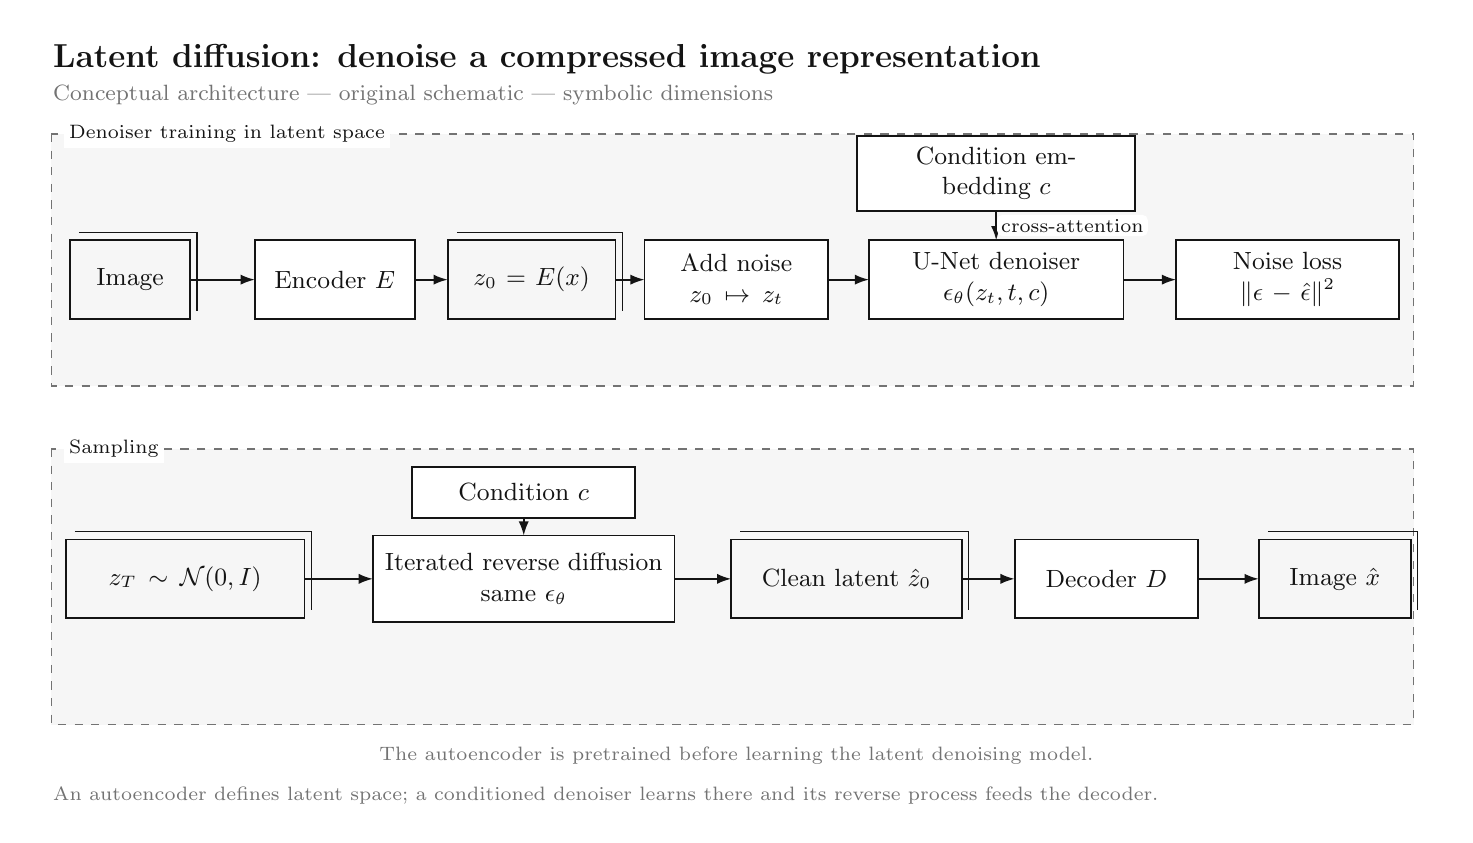
\begin{tikzpicture}[x=1cm,y=-1cm,font=\rmfamily,text=ink]

\path[use as bounding box] (0,0) rectangle (18,10);
\node[anchor=west,font=\large\bfseries] at (.2,.4) {Latent diffusion: denoise a compressed image representation};
\node[anchor=west,font=\footnotesize,text=soft] at (.2,.85) {Conceptual architecture | original schematic | symbolic dimensions};
\begin{pgfonlayer}{background}
\draw[groupbox] (0.3,1.35) rectangle (17.6,4.550000000000001);
\node[anchor=west,font=\scriptsize,fill=white,inner sep=2pt] at (0.44999999999999996,1.35) {Denoiser training in latent space};
\draw[groupbox] (0.3,5.35) rectangle (17.6,8.85);
\node[anchor=west,font=\scriptsize,fill=white,inner sep=2pt] at (0.44999999999999996,5.35) {Sampling};
\end{pgfonlayer}
\node[box,fill=wash,minimum width=1.5cm,minimum height=1.0cm,text width=1.25cm] (x) at (1.3,3.2) {Image};
\draw[ink,line width=.4pt] (0.65,2.6) -- (2.15,2.6) -- (2.15,3.6);
\node[box,minimum width=2.0cm,minimum height=1.0cm,text width=1.75cm] (e) at (3.9,3.2) {Encoder $E$};
\node[box,fill=wash,minimum width=2.1cm,minimum height=1.0cm,text width=1.85cm] (z0) at (6.4,3.2) {$z_0=E(x)$};
\draw[ink,line width=.4pt] (5.45,2.6) -- (7.55,2.6) -- (7.55,3.6);
\node[box,minimum width=2.3cm,minimum height=1.0cm,text width=2.05cm] (q) at (9.0,3.2) {Add noise\\$z_0\mapsto z_t$};
\node[box,minimum width=3.2cm,minimum height=1.0cm,text width=2.95cm] (u) at (12.3,3.2) {U-Net denoiser\\$\epsilon_\theta(z_t,t,c)$};
\node[box,minimum width=2.8cm,minimum height=1.0cm,text width=2.55cm] (loss) at (16.0,3.2) {Noise loss\\$\|\epsilon-\hat\epsilon\|^2$};
\node[box,minimum width=3.5cm,minimum height=0.65cm,text width=3.25cm] (cond) at (12.3,1.85) {Condition embedding $c$};
\node[box,fill=wash,minimum width=3.0cm,minimum height=1.0cm,text width=2.75cm] (zt) at (2.0,7.0) {$z_T\sim\mathcal N(0,I)$};
\draw[ink,line width=.4pt] (0.6,6.4) -- (3.6,6.4) -- (3.6,7.4);
\node[box,minimum width=3.8cm,minimum height=1.1cm,text width=3.55cm] (rev) at (6.3,7.0) {Iterated reverse diffusion\\same $\epsilon_\theta$};
\node[box,fill=wash,minimum width=2.9cm,minimum height=1.0cm,text width=2.65cm] (zh) at (10.4,7.0) {Clean latent $\hat z_0$};
\draw[ink,line width=.4pt] (9.05,6.4) -- (11.95,6.4) -- (11.95,7.4);
\node[box,minimum width=2.3cm,minimum height=1.0cm,text width=2.05cm] (d) at (13.7,7.0) {Decoder $D$};
\node[box,fill=wash,minimum width=1.9cm,minimum height=1.0cm,text width=1.65cm] (out) at (16.6,7.0) {Image $\hat x$};
\draw[ink,line width=.4pt] (15.750000000000002,6.4) -- (17.650000000000002,6.4) -- (17.650000000000002,7.4);
\node[box,minimum width=2.8cm,minimum height=0.65cm,text width=2.55cm] (c2) at (6.3,5.9) {Condition $c$};
\begin{pgfonlayer}{background}
\draw[flow] (x.east) -- (e.west);
\draw[flow] (e.east) -- (z0.west);
\draw[flow] (z0.east) -- (q.west);
\draw[flow] (q.east) -- (u.west);
\draw[flow] (u.east) -- (loss.west);
\draw[flow] (cond.south) -- (u.north) node[midway,right,fill=white,inner sep=1.5pt,font=\scriptsize] {cross-attention};
\draw[flow] (zt.east) -- (rev.west);
\draw[flow] (rev.east) -- (zh.west);
\draw[flow] (zh.east) -- (d.west);
\draw[flow] (d.east) -- (out.west);
\draw[flow] (c2.south) -- (rev.north);
\end{pgfonlayer}
\node[annotation,text width=14cm] at (9,9.25) {The autoencoder is pretrained before learning the latent denoising model.};
\node[anchor=west,align=left,font=\scriptsize,text=soft,text width=17.6cm] at (.2,9.75) {An autoencoder defines latent space; a conditioned denoiser learns there and its reverse process feeds the decoder.};
\end{tikzpicture}
\end{document}
